\chapter{Problematik und Lösungsansätze}

In den letzten Jahren wurden einige Arbeiten über mobile Anwendungsentwicklung und auch Cross-Plattform, beziehungsweise hybride Anwendungsentwicklung veröffentlicht. In der Arbeit von X und Y (Comparison of Cross-Platform Mobile Development(X)) von 2012 wurden die 4 Frameworks Rhodes, PhoneGap, DragonRad and MoSync miteinander verglichen. Bei ihrer Arbeit konnten sie folgende Vorteile bei der hybriden Anwendungsentwicklung ausmachen: 

\begin{itemize}
\item Reduzierung der benötigten Skills: Hybride Frameworks verwenden meist gängige Programmiersprachen wie HTML oder JavaScript.
\item Weniger Code: Da plattformübergreifender Code produziert wird, muss nicht mehr für jede Plattform eine eigene komplette Anwendung mit separater Codebase entwickelt werden.
\item Reduzierung der Entwicklungszeit und Wartungskosten, da nur eine Anwendung entwickelt und gewartet werden muss im Vergleich zu mehreren nativen Anwendungen. 
\item Die Entwickler müssen sich in weniger APIs einarbeiten und sich auskennen, da nicht direkt mit den APIs der Plattformen gearbeitet wird, sondern mit der API des jeweiligen Framework.
\item Wachsende Marktanteile für das Business hinter der Anwendung. 
\end{itemize}

Zusammengefasst lässt sich sagen, dass die hybride Anwendungsentwicklung einerseits verspricht die Investitionskosten zu senken und andererseits den Verkauf der Anwendungen auf mehrere Märkte ausweitet. Die Bewertungskriterien, anhand derer X und Y die Frameworks in ihrer Arbeit evaluiert haben, waren folgende: 

\begin{itemize}
\item Die Betriebssysteme, die von den Frameworks unterstützt werden
\item Lizenzen für die Frameworks zur Evaluierung der Geschäftsbedingungen
\item Verfügbare Programmiersprachen für die Entwicklung der Anwendungen
\item Verfügbarkeit der APIs hinsichtlich der Fragestellungen welche nativen Funktionen genutzt werden können
\item die Architektur, die für den Entwicklungsprozess der Anwendung zur Verfügung steht
\item Integrated Development Environments (IDEs) die verfügbar und nutzbar sind
\end{itemize}

Für die API-Tests hat sich für die 4 von X und Y ausgewählten Frameworks folgendes Bild ergeben(Abbildung \ref{fig:Ergebnis_API_Test_Publ}): 

\begin{figure}[h]
	\centering
	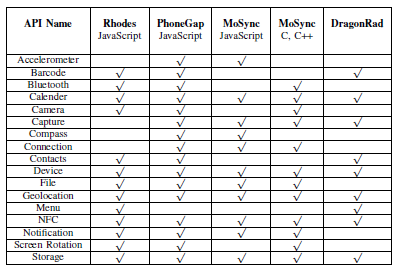
\includegraphics[width=0.7\textwidth]{Bilder/Ergebnis_Sensornutzung_Comparison_of_Cross-Platform_Mob_Dev.PNG}
	\caption{Ergebnis API-Tests aus X und Y Arbeit: Comparison of Cross-Platform Mobile Development aus 2012}
	\label{fig:Ergebnis_API_Test_Publ}
\end{figure}

Wie man in Abbildung \ref{fig:Ergebnis_API_Test_Publ} erkennen kann, schafft es vor allem PhoneGAp alle bis auf eine getestete native Funktionalität umzusetzen. Allerdings fanden X und Y heraus, dass vor allem die Frameworks, welche auf JavaScript basieren, deutliche Performance-Probleme haben. Aus diesem Grund raten die Autoren davon ab JavaScript-basierte Frameworks für Anwendungen mit komplexen Funktionalitäten oder im Hintergrund laufende Services zu nutzen. Auch sei die Unterstützung von High-End Grafiken und 3D-Technologien unzureichend. 
\\
\\
Eine weitere Arbeit, die sich mit dem Vergleich von hybriden Frameworks beschäftigt hat ist die von X und Y: Cross-Platform Mobile Development: A Study on Apps with Animations(X) aus dem Jahr 2014. Die Frameworks, die in dieser Arbeit evaluiert wurden sind MoSync, Titanium, JQuery \& JQuery Mobile und PhoneGap. Die Bewertungskriterien, die die Autoren aufstellten sind folgende:

\begin{itemize}
\item Lizenzmodell und Kosten
\item Die Vielfältigkeit und Qualität der verfügbaren APIs
\item Das Angebot an Tutorials
\item Die Größe der Community
\item Die Komplexität des Codes um die vorgegebene Anwendung zu implementieren
\item Die Benutzerfreundlichkeit der IDE des Frameworks
\item Die Liste der unterstützten Geräte
\item Inwieweit die Frameworks das Erstellen einer nativen Benutzeroberfläche unterstützen 
\item Das geforderte Basiswissen im Bereich Programmierung und Technologiekenntnis für jedes Framework
\end{itemize}

Wie man an den Bewertungskriterien oben schon erkennen kann, gaben die Autoren eine Beispiel-Anwendung vor, die mit Hilfe der 4 ausgewählten Frameworks implementiert wurde, um diese gegeneinander zu evaluieren. Um einem Bias entgegenzuwirken wurden für die einzelnen Entwicklungen Entwickler ausgewählt, die mit der jeweiligen Programmiersprache bereits vertraut waren. Die Frameworks wurden anschließend in den oben aufgeführten Kategorien mit Noten von 0 (schlecht) bis 5 (sehr gut) bewertet. Unten stehende Tabelle (Abbildung (X)) zeigt die Ergebnisse:

 \begin{figure}[h]
	\centering
	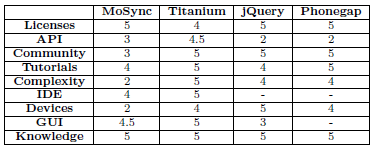
\includegraphics[width=0.65\textwidth]{Bilder/Ergebnis_Framework_Bewertung_Publ_2.PNG}
	\caption{Ergebnis Framework Evaluation von X und Y: Cross-Platform Mobile Development: A Study on Apps with Animations aus 2014}
	\label{fig:Ergebnis_API_Test_Publ}
\end{figure}

Auf Basis oben (Abbildung (X)) dargestellten Ergebnisses bewerten die Autoren das Framework Titanium als das Bestes unter den getesteten für Anwendungen mit Animationen. Begründung hierfür ist, dass Titanium Animationen und Übergangseffekte nativ unterstützt und die Performance gut ist und vermuten lässt, dass auch bei komplexeren Anwendungen die Performance noch ausreichend sein wird. 
\\
\\
In dieser Arbeit sollen ebenfalls, wie bei oben vorgestellten Publikationen, hybride Frameworks direkt miteinander verglichen werden. Um die zu evaluierenden Frameworks auszuwählen, wird zunächst eine Marktanalyse durchgeführt, welche anzeigen soll, welche Frameworks die aktuell attraktivsten sind. Für die Evaluation wird eine Test-Anwendung entwickelt, die mit den ausgewählten Frameworks implementiert werden soll. Diese Anwendung wird zuvor noch als Referenz für zum Beispiel die Performance noch nativ implementiert. Die Anzahl der Frameworks, die mit dieser Anwendung getestet werden ist dabei auf 5 limitiert. Allerdings werden noch weitere Frameworks mit in die Evaluation aufgenommen. Diese können aber nur nach Bewertungskriterien verglichen werden, die nicht direkt mit dem Entwicklungsprozess zusammenhängen. Es wird versucht die Kriterienkataloge der oben vorgestellten Publikationen mittels einer Umfrage unter Anwendungsentwicklern noch zu erweitern. Da aufgrund bisheriger Publikationen davon auszugehen ist, dass es nicht 'das eine' Framework für alle Problemstellungen gibt, soll das Ergebnis dieser Arbeit ein Entscheidungsbaum werden, anhand dessen das ideale Framework je Problematik ermittelt werden kann. 

